\section{Algorithme polynomial pour une capacité infinie}

\subsection{Modèle et hypothèses}

\begin{frame}[label=CapaciteInfinie]
  \frametitle{Modèle et hypothèse}
  
  \begin{center}
  
    \begin{minipage}[c]{.5\linewidth}
      \begin{center}
        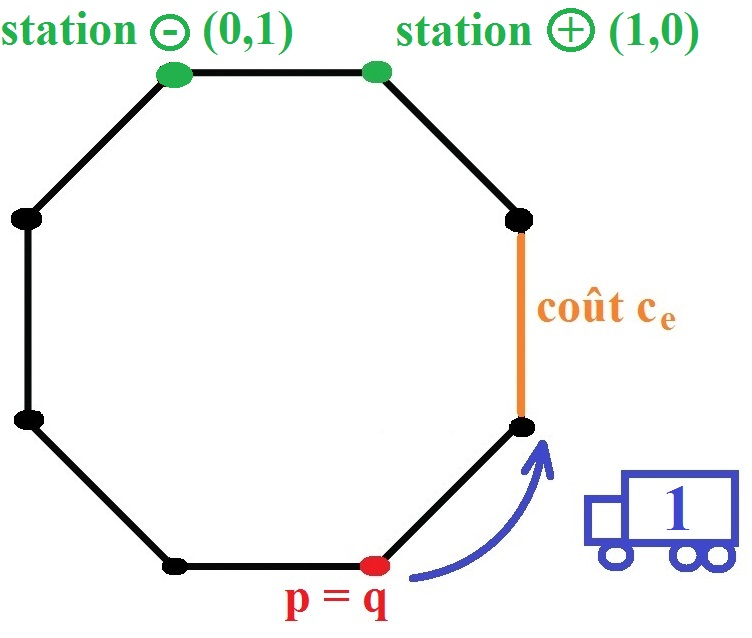
\includegraphics[width=\textwidth]{CapaciteInfinie/modele.jpg}
      \end{center}
    \end{minipage}\hfill
    \begin{minipage}[c]{.5\linewidth}
      \textbf{Hypothèses :}
      \begin{itemize}
      \item Capacité de transport $C$ infinie
      \item $p=q$
      \end{itemize}
    \end{minipage}
    
  \end{center}

\end{frame}

\subsection{Algorithme}

\begin{frame}[label=AlgoCapaciteInfinie]
  \frametitle{Idée générale de l'algorithme}
  \begin{center}
    \begin{minipage}[c]{\linewidth}
      \begin{minipage}[c]{.2\linewidth}
        \begin{overlayarea}{\textwidth}{0.28\textheight}
          \only<1>{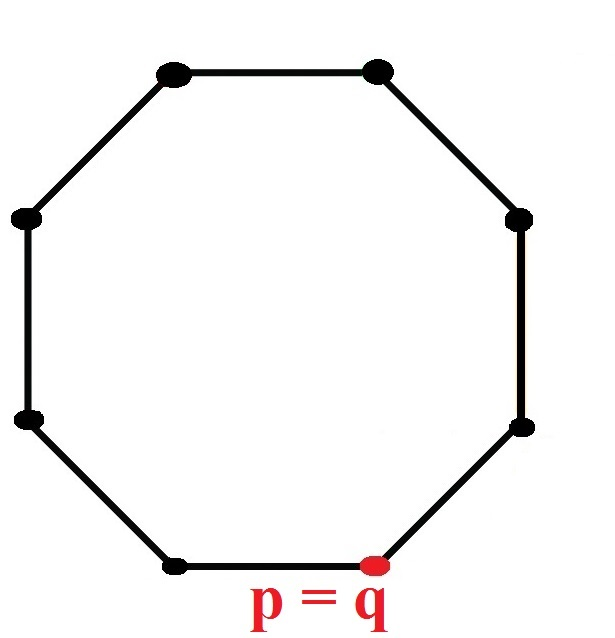
\includegraphics[width=\textwidth]{CapaciteInfinie/GrapheG.jpg}}
          \only<2>{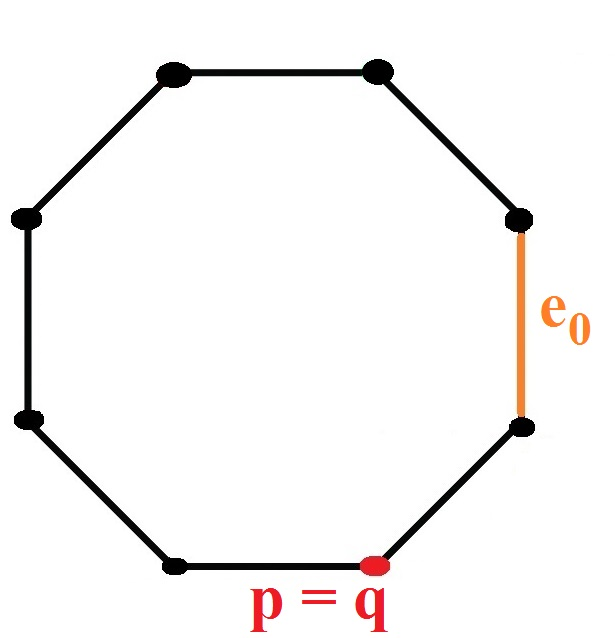
\includegraphics[width=\textwidth]{CapaciteInfinie/e0.jpg}}
          \only<3->{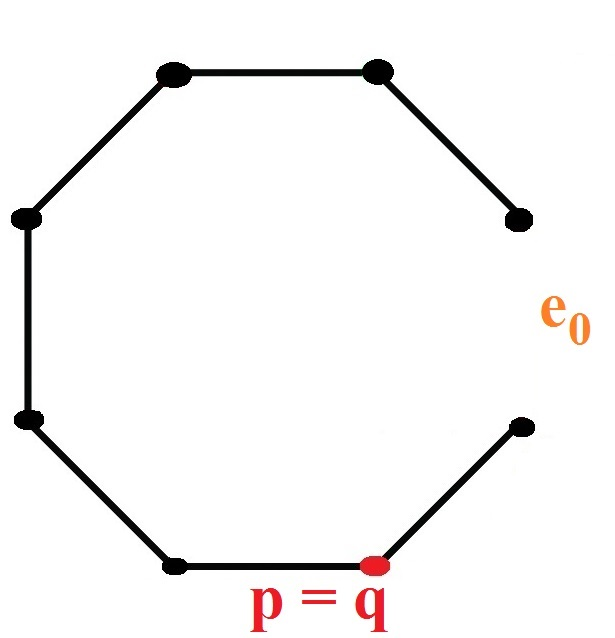
\includegraphics[width=\textwidth]{CapaciteInfinie/suppr_e0.jpg}}
        \end{overlayarea}
      \end{minipage}
      \begin{minipage}[c]{.8\linewidth}
        \begin{overlayarea}{\textwidth}{0.28\textheight}
          \begin{itemize}
          \item<2-> Pour chaque $e_0 \in E$
            \begin{enumerate}
            \item<3-> Construire $\bs{G(e_0)}$ en supprimant $e_0$
            \item<4-> Résoudre le SSBP sur $\bs{G(e_0)}$\\
            (algorithme dans le cas linéaire)
            \end{enumerate}
          \end{itemize}
        \end{overlayarea}
      \end{minipage}
    \end{minipage}
    \begin{minipage}[c]{\linewidth}
      \begin{minipage}[c]{.2\linewidth}
        \begin{overlayarea}{\textwidth}{\textheight}
          \only<5>{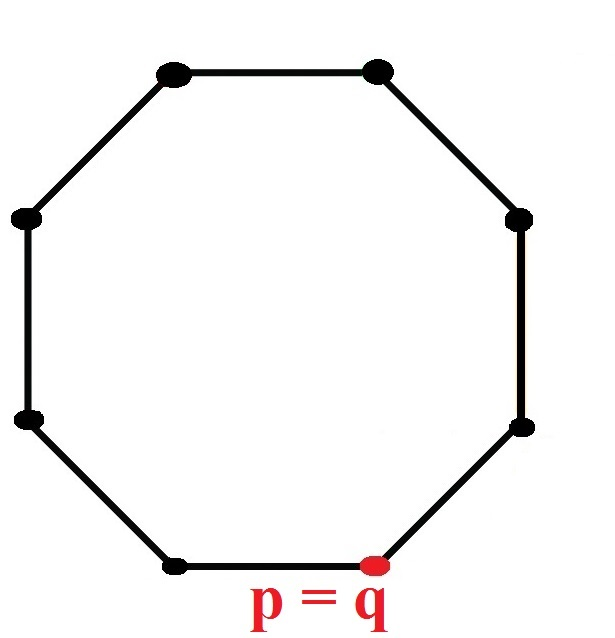
\includegraphics[width=\textwidth]{CapaciteInfinie/GrapheG.jpg}}
          \only<6>{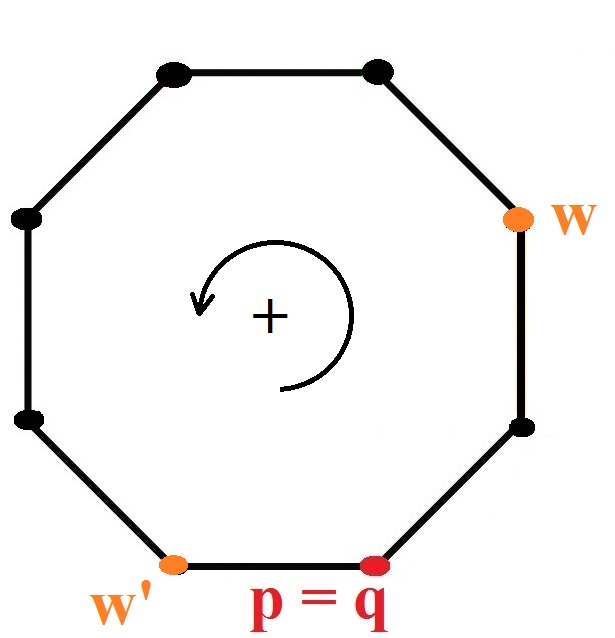
\includegraphics[width=\textwidth]{CapaciteInfinie/w.jpg}}
          \only<7>{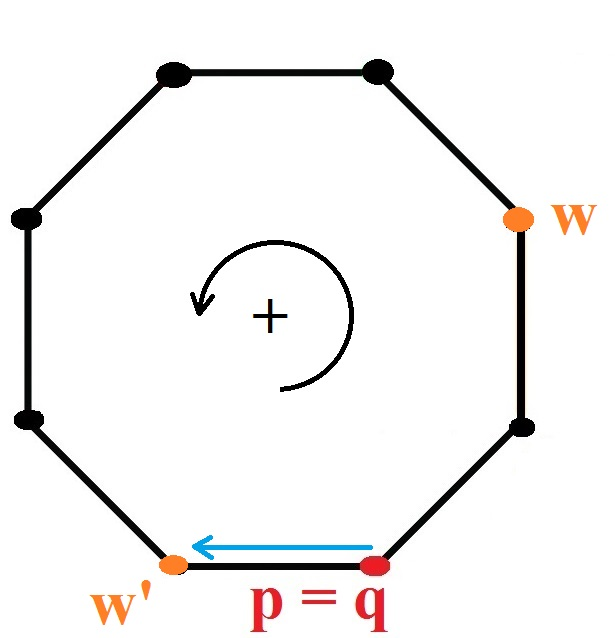
\includegraphics[width=\textwidth]{CapaciteInfinie/w_1.jpg}}
          \only<8>{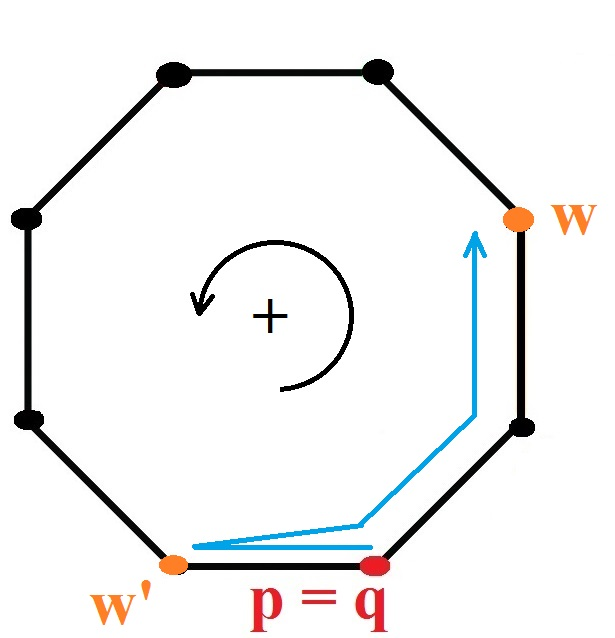
\includegraphics[width=\textwidth]{CapaciteInfinie/w_2.jpg}}
          \only<9>{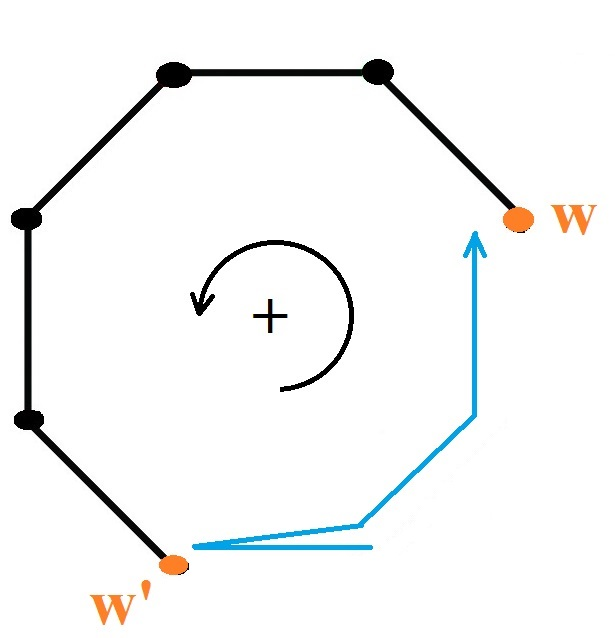
\includegraphics[width=\textwidth]{CapaciteInfinie/w_3.jpg}}
          \only<10>{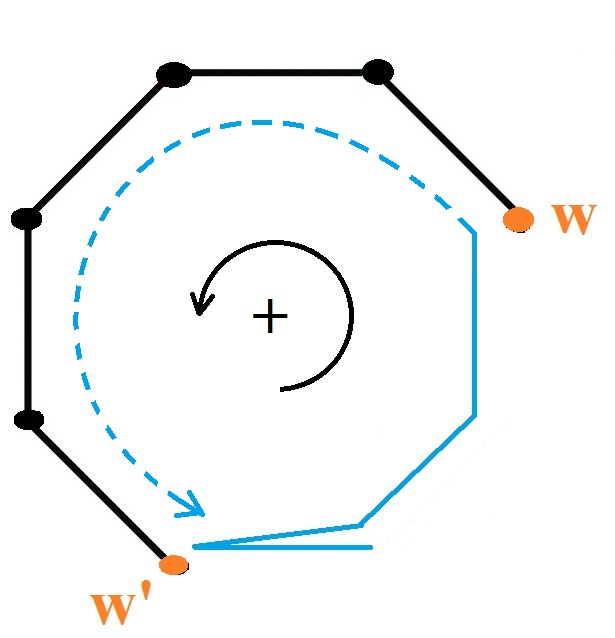
\includegraphics[width=\textwidth]{CapaciteInfinie/w_4.jpg}}
          \only<11>{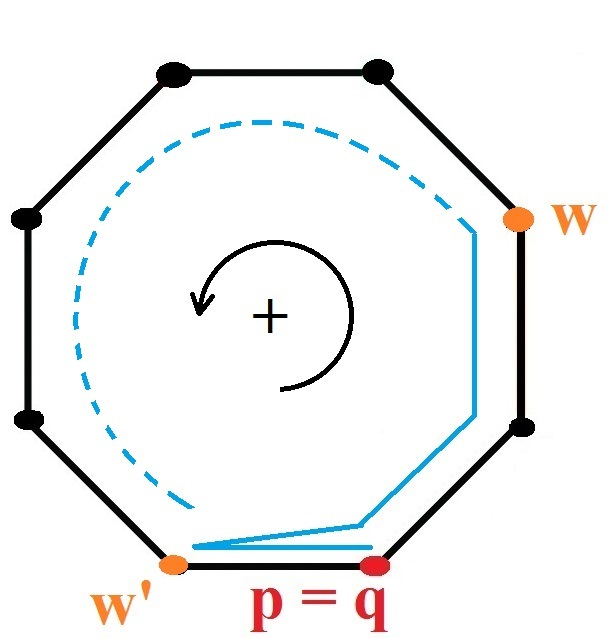
\includegraphics[width=\textwidth]{CapaciteInfinie/w_5.jpg}}
          \only<12>{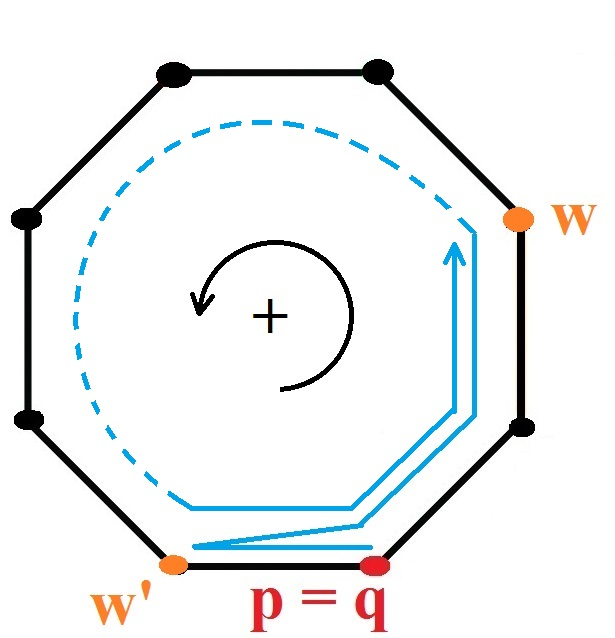
\includegraphics[width=\textwidth]{CapaciteInfinie/w_6.jpg}}
          \only<13->{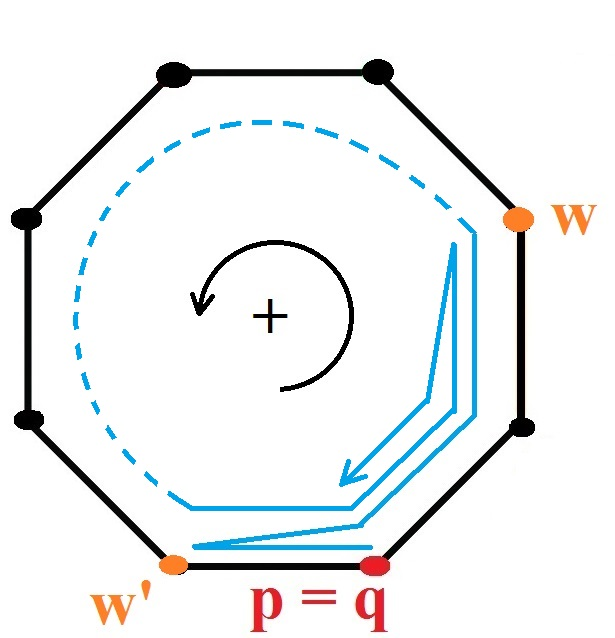
\includegraphics[width=\textwidth]{CapaciteInfinie/w_7.jpg}}
        \end{overlayarea}
      \end{minipage}
      \begin{minipage}[c]{.8\linewidth}
        \begin{overlayarea}{\textwidth}{\textheight}
          \begin{itemize}
          \item<6-> Pour chaque $w \in V$, pour chaque $w' \in ]w,p]_+$
            \begin{enumerate}
            \item<7-> aller jusqu'à $w'$ dans le sens $(-)$
            \item<8-> aller jusqu'à $w$ dans le sens $(+)$ en ramassant tous les vélos
            \item<9-> Construire le graphe linéaire $\bs{G(w,w',+)}$
            \item<10-> Résoudre le SSBP sur $\bs{G(w,w',+)}$\\
            (algorithme dans le cas linéaire)
            \item<12-> aller jusqu'à $w$ dans le sens $(+)$ en équilibrant toutes les stations
            \item<13-> revenir en $p$ dans le sens $(-)$
            \end{enumerate}
          \item<14-> Faire de même en allant d'abord sur $w$ dans le sens $(+)$
          \end{itemize}
        \end{overlayarea}
      \end{minipage}
    \end{minipage}
  \end{center}
\end{frame}

\begin{frame}[label=OptimaliteCapaciteInfinie]
  \frametitle{Complexité du cas de la capacité infinie}

  \begin{thm} \label{thm: optimalité algo infini}
  Il existe une algorithme cubique en le nombre de sommets résolvant le SSBP dans le cas où $C$ est infinie et où $p=q$.

  De plus, le coût $\Upsilon_{G}$ de la solution optimale est donnée par le minimum entre
  $$
    \min_{e \in E} \Upsilon_{G(e)}
  $$
  et
  $$
    \min_{w \in V, w' \in ]w,o]_+}
    \left(
      3 \sum_{ e \in E\left[ \left[w',w\right]_+ \right] }c_e + \min \left( \Upsilon_{G(w,w',+)} , \Upsilon_{G(w,w',-)} \right)
    \right)
  $$
  \end{thm}
\end{frame}

\begin{frame}
  \frametitle{Démonstration de la complexité du cas de la capacité infinie}
  \framesubtitle{Restriction du nombre de passages sur une arête particulière}

  \begin{overlayarea}{\linewidth}{\columnwidth}
  \only<1->{
  \begin{lem} \label{lem: passe au plus une fois par e0}
  Soit $S$ une solution optimale du SSBP dans le cas où $C$ est infinie et où $p=q$. Alors il existe une arrête $e_0 \in E$ tel que le camion passe au plus une fois par $e_0$.
  \end{lem}
  }
  \only<2->{
    \begin{proof}
      \begin{itemize}
        \item<3-> $\mbox{Coût}(S) < 2\sum_{e \in E}c_e$
        \item<4-> Par l'absurde, on ne peut passer deux fois par chaque arête.
      \end{itemize}
      \vskip-1\baselineskip
    \end{proof}
  }
  \end{overlayarea}
\end{frame}

\begin{frame}
  \frametitle{Démonstration de la complexité du cas de la capacité infinie}
  \framesubtitle{Restriction du nombre de passages sur l'ensemble des arêtes}
  
  \begin{lem} \label{lem: passe au plus 3 fois par chaque e}
  Soit $G=(V,E)$ un graphe circulaire. On suppose que la capacité $C$ du camion est infinie et que $p=q$.\\
  Alors il existe une solution réalisable optimale telle que :\\
  pour toute arête $e \in E$, le camion passe au plus trois fois sur $e$.
  \end{lem}

\end{frame}

\begin{frame}
  \frametitle{Démonstration de la complexité du cas de la capacité infinie}
  \framesubtitle{[Démonstration] Restriction du nombre de passages sur l'ensemble des arêtes}
  \onslide<1->
  {
    \begin{itemize}
    \item<1-> Deux cas :
      \begin{itemize}
      \item<2-> il existe $e_0 \in E$ tel que le camion ne passe pas par $e_0$
      \item<3-> le camion passe par tous les sommets et\\
      il existe $e_0 \in E$ tel que le camion passe exactement une fois par $e_0$
      \end{itemize}
    \end{itemize}
  }
  \onslide<4->
  {
    \begin{center}
      \onslide<4->
      {
        \begin{minipage}[c]{.4\linewidth}
        \begin{center}
          Solution initiale $S$\\
          \begin{overlayarea}{\textwidth}{\textheight}
            \only<4-5>{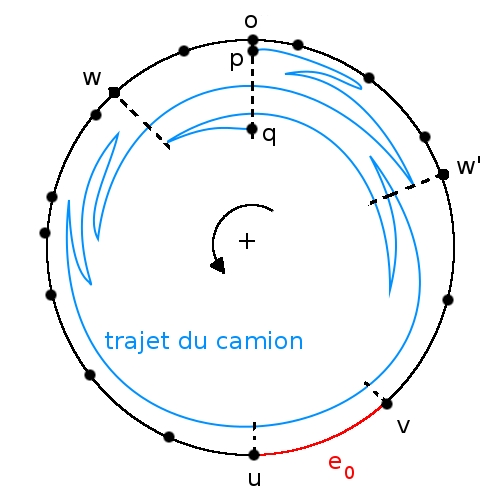
\includegraphics[width=\textwidth]{CapaciteInfinie/PreuveZeInf3.jpg}}
            \only<6>{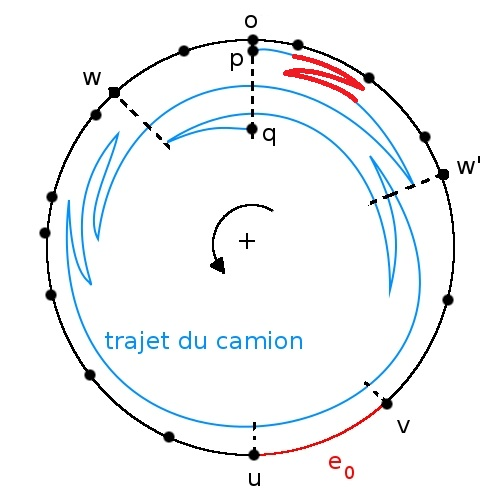
\includegraphics[width=\textwidth]{CapaciteInfinie/PreuveZeInf3_Zone1.jpg}}
            \only<7>{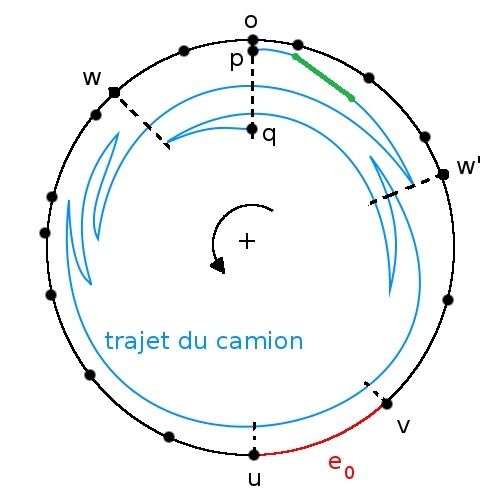
\includegraphics[width=\textwidth]{CapaciteInfinie/PreuveZeInf3_Zone1cor.jpg}}
            \only<8>{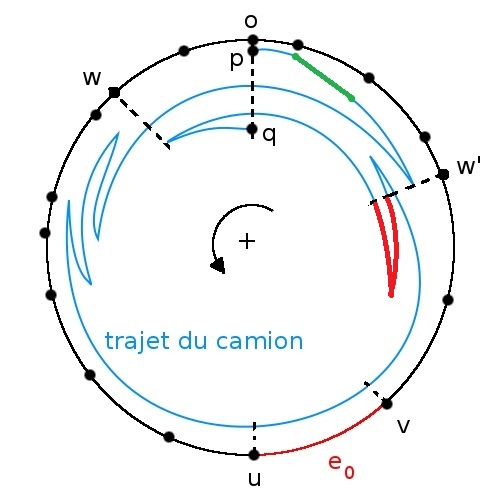
\includegraphics[width=\textwidth]{CapaciteInfinie/PreuveZeInf3_Zone2.jpg}}
            \only<9>{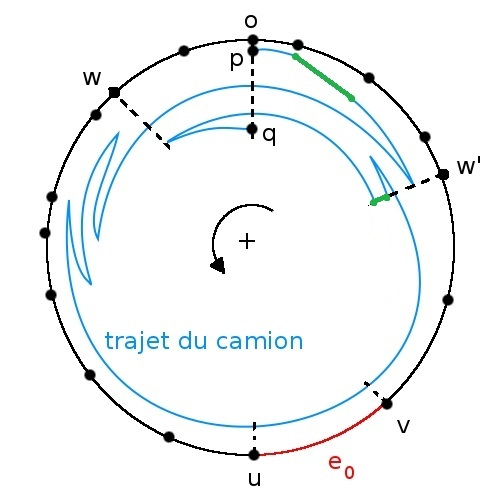
\includegraphics[width=\textwidth]{CapaciteInfinie/PreuveZeInf3_Zone2cor.jpg}}
            \only<10>{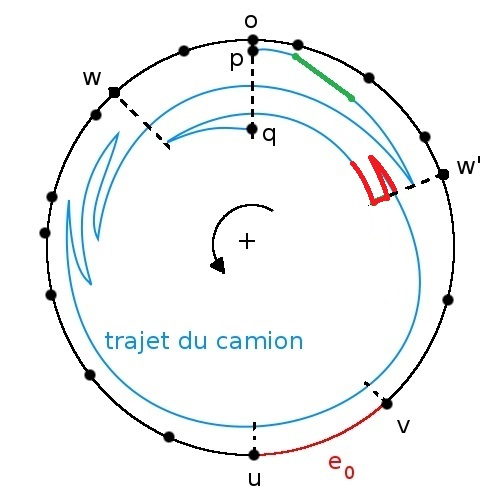
\includegraphics[width=\textwidth]{CapaciteInfinie/PreuveZeInf3_Zone3.jpg}}
            \only<11->{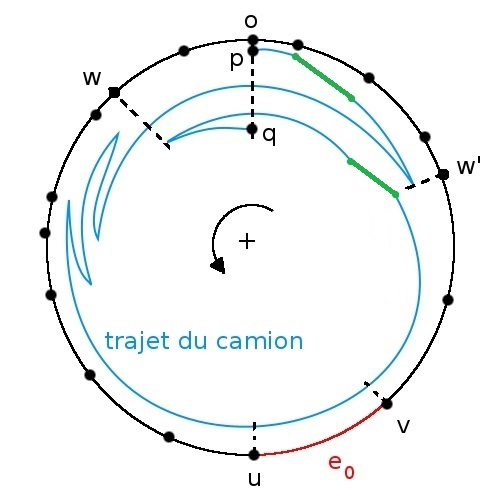
\includegraphics[width=\textwidth]{CapaciteInfinie/PreuveZeInf3_Zone3cor.jpg}}
          \end{overlayarea}
        \end{center}
        \end{minipage} \hfill
      }
      \onslide<5->
      {
        \begin{minipage}[c]{.4\linewidth}
        \begin{center}
          Nouvelle solution $S'$\\
          \begin{overlayarea}{\textwidth}{\textheight}
            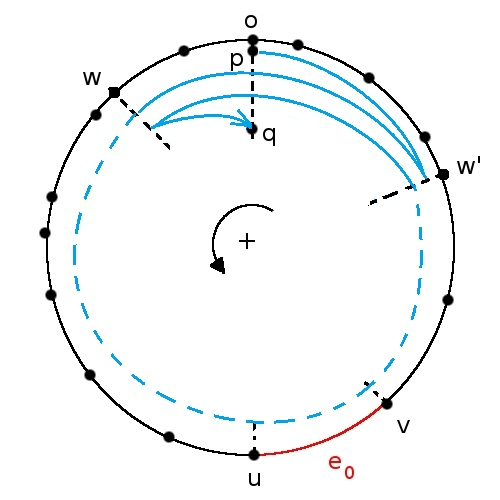
\includegraphics[width=\textwidth]{CapaciteInfinie/PreuveZeInf3_simple.jpg}
          \end{overlayarea}
        \end{center}
        \end{minipage} \hfill
      }
    \end{center}
  }
\end{frame}
